\chapter{Rhetorical Strategies}

\section{Methodology}
This work will draw upon previous efforts by Rich \cite{rich12, rich14} and Sin \cite{sin}, who each used data drawn from a decade of articles from the English-language website for the KCNA (North Korea's ruling party's official news source intended for foreign eyes) to track trends in the DPRK's nuclear rhetoric. The KCNA website is an extremely useful source of information on the views and policies of the North Korean government. It is produced directly by the government for foreign consumption, which means that patterns found within its rhetoric reveal (intentional or accidental) agenda signaling by the North Korean government rather than the biases of foreign translators \cite{rich12}. Trends discovered within these data will be compared across escalatory cycles in order to understand the way in which North Korean rhetoric tracks with the state of nuclear diplomacy.

Since the range of data Rich and Sin examine ends before the 2013 nuclear test, the rhetoric surrounding that test will be examined using the STALIN (STatistical Analyzer of Language In North Korean Propaganda) search engine, which searches all KCNA articles from the end of 1996 through mid-2015 and provides frequencies for words and phrases by month \cite{stalin}. Though STALIN's frequency analysis is far more simplistic than the regression testing done by Rich or Sin, it will provide a good indicator for basic trends. Additionally, the results of searching STALIN for the phrases used by Rich to indicate nuclear topics (any variant of the word ``nuclear" or ``nuke") for other key time periods and comparing the STALIN results to Rich's conclusions may illuminate the difference between the two methods.

No automated content analysis exists for similar statements from the United States, in part due to the significantly broader set of statements available, and producing such analysis is too complex an undertaking for this thesis. However, this does not preclude rhetorical analysis of the American side of the picture. A number of academics have analyzed the way American policy towards the DPRK has shifted over time, and the role of verbal hostility (or lack thereof) in this process.

Bleiker \cite{bleiker}, Harnisch \cite{harnisch}, Huntley \cite{huntley}, and Sigal \cite{sigal} each identify the dominant modes of discourse in American political circles about the DPRK for a different time period around the turn of the 21st century. Bleiker and Harnisch draw comparisons between diplomacy under the Clinton administration and that taking place during the early Bush years, Huntley examines the Bush years after the Agreed Framework's collapse, and Sigal (published before Bush took office) focuses on the Clinton era and before. Several other authors \cite{crs13,green} have engaged in similar examinations on the Obama administration. All attempt to trace patterns of American behavior in a way that is instructive in painting a picture of the broader rhetorical strategies employed by the United States on this issue.

The sort of qualitative analysis that is available on the American side of the US-DPRK divide is somewhat different in its utility than the numerical data that dominate the literature on North Korean rhetoric. It is, by nature, more prone to biases introduced by the authors of papers seeking to interpret it. However, this is a necessary feature of the fundamental difference in the record of public statements by American and North Korean officials. For one thing, the sheer breadth of information available from American politicians makes numerical analysis unreasonable. Additionally, the sort of statements available from American politicians - interviews once they leave power, leaked documents meant to remain private, and the like - allows discernment of political agenda in a more direct manner than the statistical tricks required to discover the reasoning behind some of the DPRK's postures. %american politicians are much worse at security than north korea, whoops

\section{North Korean Rhetoric}
\subsection{Time-Invariant}
Rich \cite{rich14} examined KCNA articles from 1997-2012 in order to develop a profile of topics and nations most frequently mentioned in conjunction with nuclear issues. In examining member nations to the six-party talks, he discovered something interesting -  the United States was near the bottom in terms of reference frequency, but was more strongly correlated with nuclear mentions than any other nation. Since the six-party talks contained the highly-involved regional players in nuclear diplomacy during the studied timeframe, it is expected that the countries party to the talks would be mentioned in a nuclear context more than other countries - however, the overwhelming focus on the United States is highly significant.

The fact that the United States is disproportionately referenced in articles discussing nuclear matters is confirmed by additional research conducted by Rich on the year of the Yeonpyeong and Cheonan incidents, during which ``increase in references to the United States, holding all else constant, [was] the largest predictor of additional references to nuclear issues" - even though in that year, references to the United States altogether were notably rarer than any other six-party talks member and barely above references to Mexico \cite{rich12}.

This suggests that, though the nuclear diplomacy effort with the DPRK is intended to be a multilateral affair, North Korea nevertheless considers the United States to be the most relevant foreign party to the conversation \cite{rich14}. This is unsurprising, as they have explicitly referenced American nuclear proliferation as the motivator and justification for their own nuclear agenda \cite{kcna, kcna3, kcna4}.

Confirming DPRK focus on the United States suggests that analyzing the nuclear issue from a primarily bilateral standpoint is in fact valid - shifting messages and the like are clearly crafted with American eyes in mind. But more generally, this provides evidence that American preference for developing broad multilateral support for negotiations is misguided - if the DPRK cares mostly about what the US thinks, adding more voices from other countries likely provides at best marginal gains.

\subsection{Time-Variant}

The articles examined primarily identified trends within the most recent half of the escalatory cycles previously discussed. During cycle 6, for example, there were a number of rhetorical shifts evident surrounding the nuclear test: Rich found that nuclear references increased leading up to the test, then declined immediately afterwards\cite{rich14}. Sin, meanwhile, noted that while most major incidents of DPRK action are framed in terms of ``nationalism", this nuclear test in particular was covered with rhetoric focused on ``US imperialism"\cite{sin}. That is, where KCNA coverage of almost every major occurrence (like missile and nuclear tests, Yeonpyeong, and Cheonan) used predominantly keywords highlighting North Korean nationalism, the 2006 nuclear test was covered using keywords highlighting US imperialism. This shift lends further credibility to the general theme of nuclear issues being seen as responses to or instigators of US action by DPRK actors.

Following the cycle 7 nuclear test, Rich found that nuclear references in KCNA articles nearly doubled - however, he still claims that his regression model shows references going down as a result of a completed nuclear test \cite{rich14}. This discrepancy may be explained by controlling for other factors - namely, the general increase of nuclear references over time, as discussed later in this section. Meanwhile, Sin identifies a deviation from the American-focused tactics seen in the previous test coverage and in Rich's conclusions - in KCNA coverage surrounding this nuclear test, frequency of rhetoric involving the international community vastly dominated the frequency of rhetoric regarding the US \cite{sin}. This suggests that the signaling effects of nuclear testing are more complicated than initially surmised.

During cycle 8, Rich's in-depth analysis of correlations between specific issues and nuclear rhetoric revealed an apparent desire on the part of the DPRK to segregate non-nuclear events and issues from the nuclear question. Indeed, coverage of the Cheonan incident and anything related to Kim Jong-un (this was during the early days of the grooming of his image for eventual leadership) was found to be the strongest negative predictor of nuclear rhetoric in KCNA articles \cite{rich12}. While coverage of Cheonan still involved a significant amount of US-centered rhetoric\cite{sin}, it would seem to be the case that this signaling is independent from and perhaps different in inspiration than the nuclear rhetoric.

The nuclear test in cycle 10 occurred several months after the endpoint of data examined by even the broadest-ranging existing KCNA content analysis\cite{rich14}. Without access to the more sophisticated software used by content analysis literature, use of the simpler frequency-aggregating STALIN engine will still provide some indication of where the rhetorical trends lead. Examining the frequency of words containing ``nuke" or ``nuclear" in the 6-month period prior to the 2013 nuclear test, the monthly average frequency was 56.8 articles. Meanwhile, in the 6-month period following the test, a monthly average of 196.7 articles containing the nuclear keywords were published. Extending the assessment period to a year in either direction, the pre-test average was 63.3 references per month, while the post-test average was 123.

The post-test decline that Rich\cite{rich14} noted in his analysis does not seem to be present in the 2013 nuclear test coverage, as monthly references almost quadrupled in shorter-term analysis, and doubled in year-long examination. It is worth noticing that in Rich's analysis also uncovered an increase in nuclear references after the 2009 nuclear test, but drew the conclusion about rhetorical draw-down regardless. It is possible that the overall trend of increasing references overwhelmed the draw-down effect of a missile test, as annual averages did increase from 7.3 in 1997 (the earliest year for which complete KCNA archives are available) to 63.9 in 2014 (the most recent year with complete archives). However, for both the 2006 and 2009 tests, pre- and post-test monthly averages at both the 6-month and 1-year benchmarks differed by at most 17\%, as compared to a nearly 50\% increase at the 1-year benchmark for the 2013 test. It is infeasible to separate the effects of single nuclear tests within the scope of this project, so the most that can be done with the information present is say that there was a dramatic increase in the number of references to nuclear matters after the 2013 test.

In addition to rhetorical shifts that correlate with escalatory cycles, there are two important turning points that did not occur during an escalatory cycle: the Axis of Evil speech and Kim Jong-il's death.

In 2002 (between cycles 3 and 4), US President George W. Bush's State of the Union speech referenced North Korea by name as part of ``an axis of evil, arming to threaten the peace of the world."\cite{sotu02} This American rhetorical flourish (which will be discussed in more detail in the following section) did not explicitly or immediately lead to direct fallout, excluding it from consideration as a precipitating incident of an escalatory cycle. However, it is correlated with a major jump in nuclear references in KCNA articles \cite{rich14} and was repeatedly used by North Korean officials as a signal of American attitudes that justified the magnitude of their actions\cite{bleiker}.

In 2003, at the tail end of cycle 4 and correlated with both the restart of the Yongbyon reactor and the first two rounds of the six-party talks, STALIN statistics indicate that the average monthly mentions of nuclear topics hit a distinct local maximum, as shown in figure \ref{fig:kcna_refs}. Immediately after this period, US officials were shown DPRK nuclear facilities. It seems likely that this uptick is explained largely by the number of parallel but not explicitly linked issues of a nuclear nature that were happening in the country during 2003 - unlike some later increases in nuclear rhetoric that are less straightforwardly mapped to time periods of high activity.

\begin{figure}
\centering
	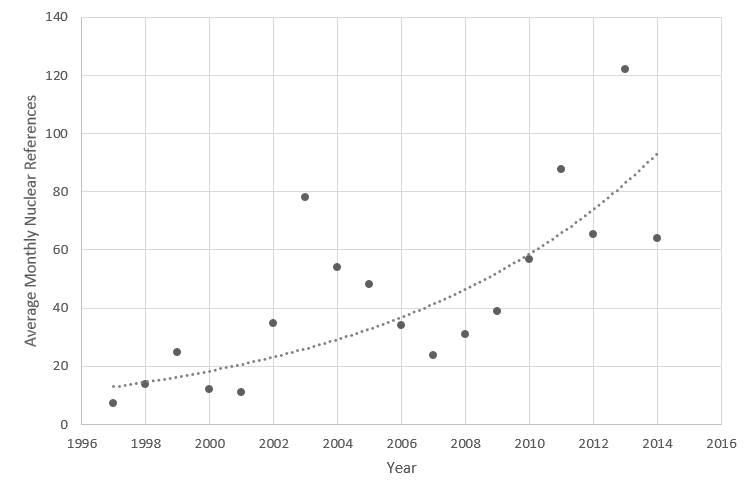
\includegraphics[width=0.7\linewidth]{../kcna_refs}
	\caption{Monthly frequency of articles using the words ``nuke" or ``nuclear" were scraped from STALIN search results. Frequencies were averaged by year. Exponential distribution produces $R^2=0.622$, which is higher than linear or any reasonable polynomial fit.}
\label{fig:kcna_refs}
\end{figure}


At the end of 2011, Kim Jong-il died and his son succeeded him as ruler of the DPRK. At this time, there was also a dramatic increase in nuclear rhetoric in KCNA articles, perhaps in an attempt to reinforce the strength of the new regime in the eyes of the international community\cite{rich14}. This also did not directly feed into an escalatory cycle, although there were obviously a great deal of secondary impacts to the changeover of power.

\subsection{Results and Trends}

The clearest trend in North Korean nuclear rhetoric has been its dramatic increase over time. This is shown in figure \ref{fig:kcna_refs}, which tracks average monthly references for each year 1997-2014. Despite an outlier in 2003, the distribution follows an upward and in fact approximately exponential trend - which tracks with the increase in distinct escalatory cycles as time passes. In general, it seems evident that the DPRK has been ramping up its nuclear ambitions, both in word and deed, at an ever-increasing rate as time passes.

The implications are concerning: the longer the status quo remains, the more emphasis will likely be placed on retaining nuclear competence, both rhetorically and materially. This is confirmed by historical examination - where earlier cycles contained agreements to roll back the DPRK's nuclear programs almost completely, it has been made clear in more recent years that this is no longer an option the DPRK will consider. The more time passes, the harder it may become to achieve the stated US objective of complete denuclearization.

The rhetoric used by North Korea to discuss nuclear tests and other significant military incidents suggests that such actions are, to some significant extent, posturing for the attention of the United States. This would seem to contraindicate the emphasis many politicians place on returning to multilateral negotiations like the six-party talks. Each additional participant in negotiations adds a new set of demands and their own agenda to the mix, and if no commensurate benefit is seen from adding more voices to the conversation, it becomes counterproductive very quickly. The modern US diplomatic strategy relies heavily upon applying pressure in conjunction with the international community, but it seems that the DPRK is uninterested in the international community's perspective on nuclear matters.


\section{American Rhetoric}
\subsection{Time-Invariant}

Bleiker \cite{bleiker} analyzed American policy with respect to the DPRK, focusing on the Clinton and Bush administrations. He found a systematic trend in the rhetoric and apparent worldview of American officials rooted in Cold War ideology - the notion of the ``rogue state". Defined oppositionally to US interests, the ``rogue state" is a foreign threat that must be thwarted at every turn. The intensity of the rhetoric couching this notion has ebbed and flowed, but the fundamental paradigm remains the same, and has been identified by many scholars\cite{bleiker,cumings,sigal,smith}.

Furthering this analysis, Smith suggests that most American politicians view North Korea as either ``mad" or ``bad" - in each case, fundamentally malicious, and either unknowable (``mad", and therefore impossible to negotiate with) or devious (``bad", and therefore morally repugnant to engage in diplomacy with). This split is evidenced by the dual focus in public statements regarding the DPRK on their instability and the grave threat they pose to the United States and its allies \cite{smith}. 

Another rhetorical factor that frequently escapes mention in analysis of this relationship is the nuclear posturing done by the United States. Ever since the 1950s, when the US violated a portion of the Korean Armistice Agreement to place nuclear weapons in South Korea, American policy has consistently erred on the side of nuclear grandstanding with respect to the DPRK \cite{cumings}. Indeed, in 1999 the DPRK had been the subject of more nuclear threats from the US than any other nation \cite{sigal}. Three years later, a leaked Defense Department report identified the nation as one of seven potential targets for nuclear strikes \cite{harnisch}.

North Korea has been intermittently labeled ``America's greatest security threat"\cite{cumings} since at least the 1990s. In conjunction with the ``rogue state" ideology and consistently aggressive nuclear posturing, this has framed the nature of US-DPRK diplomacy for the entire timeframe of interest with respect to the escalatory cycles.

\subsection{Time-Variant}

During the years leading up to and including cycle 1, American politicians did not seriously believe in the possibility of a diplomatic solution to the North Korean nuclear dilemma. Consequently, the prospect of negotiations was talked around and avoided, and the language of diplomacy was always heavily couched in threats \cite{sigal}.

During cycle 2, as the conflict between the US and the DPRK escalated, the former insisted upon ``crime-and-punishment"-style diplomacy \cite{bleiker}, a regime in which the DPRK would have to back down and admit wrongdoing to avoid serious negative repercussions. Former president Carter's back-channel negotiations took a different approach - encouraging cooperation and offering concessions in exchange for a rollback in the North Korean nuclear program \cite{sigal}.

In 1999, as cycle 3 was drawing to a close, a number of influential reports were published emphasizing the importance of a new, 'integrated' negotiation strategy. The Perry report, commissioned by President Clinton, advised building upon previous success with the Agreed Framework and drawing down negative incentives in parallel - rejecting status quo pressure-first diplomacy as non-sustainable and vulnerable to collapse in future crises \cite{perry}. The Armitage report, compiled by a number of individuals from the (H.W.) Bush-era Department of Defense, also advised acknowledging the place of serious diplomatic negotiations as a tool for dealing with the DPRK. The Armitage report, however, was far more critical of the Agreed Framework - casting it as a necessary but insufficient step in pursuing disarmament, but stopping short of advocating its dissolution \cite{armitage}. Meanwhile, Republican voices in Congress put pressure on the Clinton administration to stick to and even toughen the status quo strategy of demanding results from the DPRK before sanction draw-down could even be considered \cite{harnisch}. 

The necessity of courting Congressional approval for US-DPRK negotiation strategies pushed American demands higher and higher as the Clinton era gave way to Bush. To complicate matters further, different messages were broadcast by various departments within the administration - while the State Department (influenced by Armitage, of the aforementioned report) broadcast willingness to treat with the DPRK in a cooperative manner, the Defense Department (led by Donald Rumsfeld, a long-time DPRK hard-liner\cite{rumsfeld}) publicly favored a more aggressive approach \cite{harnisch}.

In early 2002, George Bush's Axis of Evil speech was a mostly-accurate indicator of the broader state of American policy views towards the DPRK. Within a few months, the Defense Department's Nuclear Posture Review was leaked, which outlined a plan for a potential nuclear strike on North Korea\cite{npreview}. Additionally, both the Posture Review and the official National Security Strategy of that year emphasized the legitimacy of pre-emptive strikes against ``rogue states"\cite{bleiker}, rhetoric that was echoed by Rumsfeld in news conferences that fall\cite{harnisch}.

Talks in North Korea in late 2002 devolved quickly to accusations of cheating on the Agreed Framework, initiating cycle 4. Diplomats from other nations reported that the American diplomatic team ``immediately started with accusations", resisting efforts at negotiation \cite{bleiker}. When the Agreed Framework collapsed and North Korea withdrew from the NPT, the Bush administration made little more than token efforts to preserve the ``line in the sand" of nonproliferation norms\cite{huntley}. Meanwhile, focus began to shift from bilateral engagement with the DPRK towards multilateral diplomacy and pressures, as the six-party talks began in late 2003 \cite{crs13}.

Bush's second inaugural address reinforced his administration's general preference for encouraging regime change in places like North Korea and avoiding diplomacy with dictators. Emphasis continued to fall on making sure nuclear weapons did not fall into the ``wrong" hands, rather than opposing proliferation in the general case - indeed, in discussing the NPT conference in 2005, a high-ranking State Department official claimed it was unreasonable to expect somewhere like the United States to make proliferation-related guarantees to somewhere like North Korea \cite{huntley}.

During cycle 5, an apparent relaxing of the previous hard-line approach during negotiations in the fourth round of six-party talks gave way to a return to the status quo. Though American negotiators made concessions on their previous stance of ``complete, verifiable, and irreversible" disarmament as a precondition to negotiation, the progress made with the Statement of Principles at the end of the talks was only brief \cite{huntley}. In early 2006, an updated National Security Strategy was released by the Bush administration, emphasizing ``proactive counterproliferation" and democracy-building \cite{nss06}. And though this document touted the successes of the six-party talks, the beginnings of a return to dogmatism is already apparent in both the preemptive strike rhetoric and in the explicit mention of the DPRK as in need of regime change \cite{nss06}.

The Obama administration began its relationship with North Korea with an eye towards more open diplomacy, echoing campaign sentiments suggesting ``willingness to engage with `rogue' governments" \cite{crs13}. In stark contrast to the Bush administration's distaste for the NPT \cite{huntley}, Obama's focus on reducing the global nuclear threat informed a renewed focus on bringing North Korea into the fold of non-proliferation norms \cite{crs13}.

The Obama administration has described its perspective as one of ``strategic patience" \cite{crs13}, though critics claim this is code for putting the North Korean nuclear issue on the back burner to all but ignore \cite{green}. The administration has continued to push for sanctions in response to incidents like the 2012 satellite launch, but the preconditions for negotiations have been reduced from ``complete, verifiable, and irreversible" disarmament \cite{huntley} to ``commit[ing] to steps toward denuclearization" \cite{crs13}.

Additionally, the Obama administration has followed the Bush lead with respect to multilateralism - pushing for a return to the six-party talks \cite{crs13}, and emphasizing a sanctioning strategy palatable to all members of the UNSC \cite{green}. This has been paired with a high degree of coordination with South Korea - from an uptick in joint military exercises to near-identical focus in diplomatic engagements \cite{crs13}.

\subsection{Results and Trends}
There is a distinct evolution in American rhetorical strategies as time has passed, largely correlated with various presidential administrations. During the Clinton administration, ``rogue state" labeling and outward hostility was combined with back-channel negotiations - perhaps seeking to preserve a sort of moral high ground while still reaping the benefits of a more conciliatory stance.

The Bush administration, by contrast, focused on acting as the world's policeman, replacing non-democratic governments with US-friendly democracies, and altering the country's nuclear agenda to make sure ``the right people" had nuclear weapons. These combined to strengthen the ``rogue state" rhetoric of the Clinton administration - going so far as to heavily imply that the radical reorganization of North Korean governmental structure would be preferable to as-is negotiation. Even back-channel diplomacy was largely replaced with all-or-nothing ultimatums, and bilateral communication was eschewed in favor of multilateral talks.

The Obama administration expanded the multilateral focus introduced by Bush - though the six-party talks fell apart in 2008, more recent years have seen significant increases in coordination between the United States and regional allies on the DPRK question. Additionally, a new emphasis on non-proliferation norms has informed the rhetorical strategies surrounding international consensus-building. In terms of direct contact with North Korean officials, ``strategic patience" has become the focus - though concessions are still demanded as preconditions to productive talks, the language such demands are couched in has been toned down dramatically.

Across administrations, the DPRK has consistently been portrayed as a ``rogue state", as unpredictable as it is dangerous. This rhetoric informs the standard bargaining position - North Korea's willingness to engage in productive diplomacy cannot be trusted until it has met substantive preconditions. The degree to which these preconditions have been emphasized has traded off from president to president, but the fundamental framework has remained. 

Interestingly, the standard bargaining position has often been subverted by back-channel negotiations and the words of some individuals within the executive branch more willing to entertain the notion of broader compromises. It seems likely that this discrepancy between public posturing and quieter action is informed at least somewhat by the need to appear responsive to public opinion - the American people tend to be displeased by the notion that their tax dollars are going towards appeasing oppressive regimes. Like the North Korea government, American politicians tend to speak in hard-line generalities in order to appear strong in their convictions, but can occasionally be induced to compromise behind closed doors.
